\documentclass[12pt]{iEEEtran}
\usepackage[utf8]{inputenc}
\usepackage{graphicx}
\usepackage[hidelinks]{hyperref}
\usepackage{indentfirst}
\usepackage[justification=centering]{caption}

\title{IFT870 - Projet de session}

\author{Louis-Vincent CAPELLI (CAPL1101) \\ 
        Tom SARTORI (SART0701) \\
        Alexandre THEISSE (THEA1804)}
\date{\today}

\begin{document}

\maketitle

% ## Data sources
% - Urban population: https://data.worldbank.org/indicator/SP.URB.TOTL
% - Total population: https://data.worldbank.org/indicator/SP.POP.TOTL
% - Country position: https://gist.github.com/tadast/8827699#file-countries_codes_and_coordinates-csv
% - Mean temperature: https://en.wikipedia.org/wiki/List_of_countries_by_average_yearly_temperature
% - COVID confirmed cases: https://www.kaggle.com/datasets/sudalairajkumar/novel-corona-virus-2019-dataset/versions/143
% - Climate classification: https://koeppen-geiger.vu-wien.ac.at/data/Koeppen-Geiger-ASCII.zip
% - Mortality rate: https://www.kaggle.com/datasets/paultimothymooney/coronavirus-covid19-mortality-rate-by-country and https://www.worldometers.info/coronavirus/

% Angles d'étude :
% Covid : 2 index :
% - Infections brutes (naïf mais peut être inclus si donne des résultats faussement convaincants)
% -> Spread : rapport d'un jour sur l'autre

% Infections par rapport à la latitude (très naïf)
% Spread par rapport à la latitude

% Spread par rapport à pop urbaine/pop totale

% Spread par rapport au climat

% Travail effectié : 
% Regrouper les DB existantes et parser les infos du web pour les mean temperatures

% Sélectionner les infos qui nous intéressent : ne garder que les données de l'année 2020, regrouper les cas par pays si nécessaire, combiner les données du monde et des US

% Sélectionner à travers les 5 fichiers les pays pour lesquels on a toutes les données en utilisant difflib pour matcher les noms des pays

% Ajout de la classification de climat pour chaque pays en choisissant le point le plus proche du centre du pays

% On a bien un nombre d'infectés par jour, c'est cumulatif

% Trouver comment calculer le spread factor et comparer avec mortality rate qui a été utilisé dans l'article


\section{Introduction}
\subsection{Titre du projet}
Analyse de la propagation du COVID-19 en fonction de la position géographique, de la part de
population urbaine et du climat. 

\subsection{Motivations}
La pandémie de COVID-19 a eu un impact majeur sur le monde entier. Les gouvernements ont dû
prendre des mesures drastiques pour limiter la propagation du virus. Cependant, la 
propagation du virus a été très inégale d'un pays à l'autre. L'objectif de ce projet 
est d'analyser les facteurs qui ont influencé la propagation du virus.

Une étude \cite{kaggle} a déjà été réalisée sur la relation entre la propagation du virus et la latitude
mais de nombreuses critiques ont mentionné qu'elle ne prenait pas assez de facteurs en compte.

Notre objectif est de réaliser une étude plus complète en prenant en compte en plus de la
position, l'urbanisation du pays et son climat comme cela a été suggeré dans les commentaires
de l'étude précédente.

\section{Données}
\subsection{Description du projet}
Le projet consiste à mettre en perspective les données de propagation du COVID-19 avec des
données géographiques, climatiques et démographiques. Le but est dans un premier temps de
retrouver les résultats de l'étude précédente \cite{kaggle} et dans un second temps de 
comparer ces résultats en prenant en compte des facteurs supplémentaires pour voir si
la position est bien un facteur déterminant dans la propagation du virus ou si elle est
simplement corrélée à d'autres facteurs plus importants.

\subsection{Contexte général}
Le COVID-19 est une maladie infectieuse causée par le coronavirus SARS-CoV-2. Elle a été
découverte en Chine en décembre 2019 et s'est rapidement propagée dans le monde entier.
Le virus se transmet par les gouttelettes respiratoires et les surfaces contaminées. Les
symptômes les plus courants sont la fièvre, la toux et la fatigue. La maladie peut être
grave et entraîner la mort, en particulier chez les personnes âgées ou souffrant de
problèmes de santé sous-jacents.

On sait que la mortalité d'un virus est fortement liée aux conditions climatiques,
la temperature par exemple pouvant être un facteur aggravant chez les personnes
les plus fragiles notamment. \cite{climate_mortality}

De plus, la densité de population est un facteur important dans la propagation d'une maladie
infectieuse puisqu'elle augmente les contacts entre les individus et donc la probabilité
de transmission du virus. C'est d'ailleurs un des facteurs à prendre en compte dans le calcule
du R0, le nombre de reproduction de base du virus. \cite{R0_wiki} \cite{sy2021population}

Ces observations nous amènent à nous poser la question de savoir si la position géographique
est vraiment une variable qui permettrait de prédire la propagation du virus ou si elle n'est qu'un
agrégat de variables plus importantes comme la densité de population ou le climat.

\subsection{Source des données}
Pour réaliser notre étude, une longue phase de collecte de données a été nécessaire. Voici les
différentes sources de données que nous avons utilisées :
\begin{itemize}
    \item \textbf{Population urbaine} : données de la Banque Mondiale \cite{urban_pop}
    \item \textbf{Population totale} : données de la Banque Mondiale \cite{total_pop}
    \item \textbf{Position géographique} : données de Tadas Talaikis \cite{country_pos}
    \item \textbf{Température moyenne} : données de Wikipedia \cite{mean_temp}
    \item \textbf{Cas confirmés de COVID-19} : données de Kaggle \cite{covid_confirmed}
    \item \textbf{Classification climatique de Köppen-Geiger} : données de l'Université de Vienne \cite{climate_classification}
    \item \textbf{Taux de mortalité} : données de Kaggle \cite{mortality_rate}
\end{itemize}

\subsection{Traitement des données}

\subsubsection{Sélection des pays étudiés}\hfill\\
Nous avons commencé par sélectionner un sous-ensemble de pays pour lesquels nous avions toutes
les données nécessaires, ce qui nous a donné un total de 159 pays.

Les pays ayant plusieurs dénominations dans les différentes bases de données, nous avons utilisé
la librairie \texttt{difflib} avec un seuil de similarité de 0.8 pour matcher les noms des pays
et ainsi pouvoir lier les données des différentes bases.
\\

\subsubsection{Position géographique}\hfill\\
La position géographique de chaque pays étant disponible dans plusieurs bases de données, nous
avons conservé les données de la base de Tadas Talaikis \cite{country_pos} qui représentent
la position moyenne des pays en latitude et longitude.
\\

\subsubsection{Climat}\hfill\\
Pour refléter le climat global d'un pays, nous avons conservé deux indicateurs : la température
moyenne et la classification climatique de Köppen-Geiger.

La température moyenne a été extraite de Wikipedia \cite{mean_temp}.

La classification
climatique de Köppen-Geiger est fournie par l'Université de Vienne \cite{climate_classification}
pour un peu plus de 90000 points répartis sur la surface du globe. 

À chaque point est associée une classe selon trois critères : le climat principal,
les précipitations et la température. Voici la répartition des classes de Köppen-Geiger
sur la surface du globe. (fig. \ref{fig:KG_classification})

\begin{figure}[h!]
    \centering
    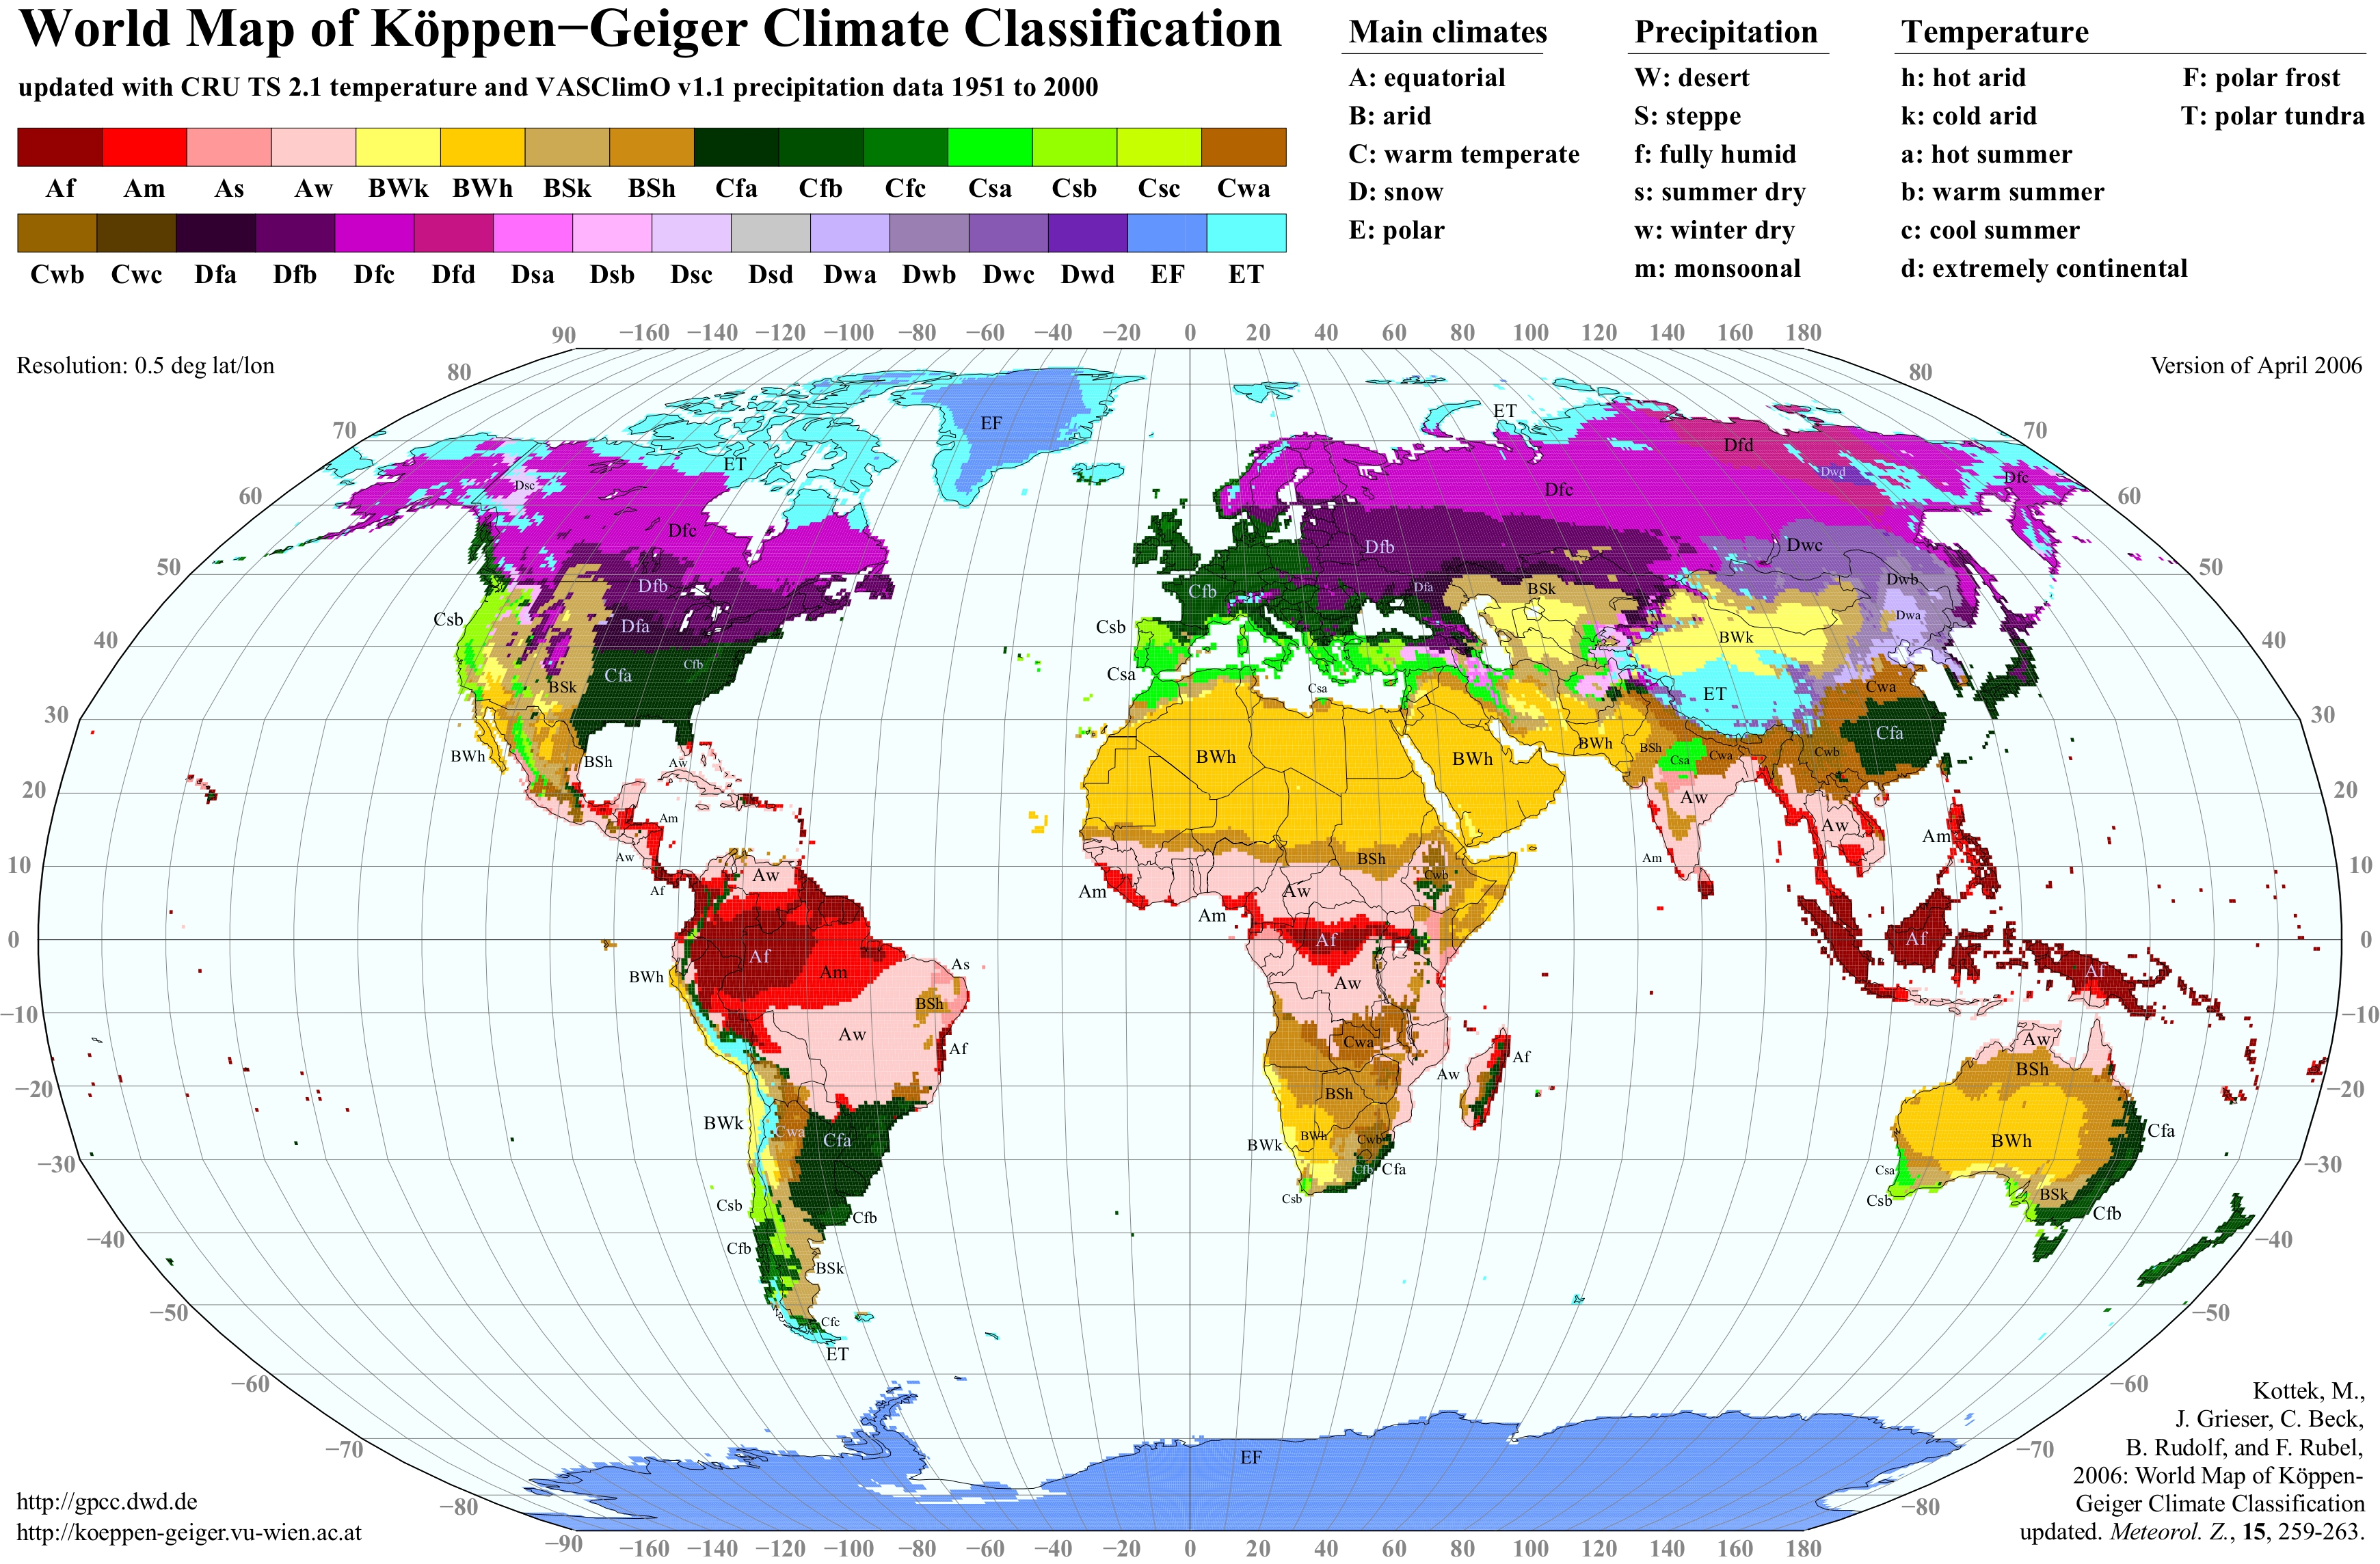
\includegraphics[width=\columnwidth]{img/KG_classification.jpg}
    \caption{Classification climatique de Köppen-Geiger}
    \label{fig:KG_classification}
\end{figure}

Nous avons calculé la distance
entre chaque pays et les points de la base de données grâce à la formule de Haversine
\cite{haversine} et avons sélectionné le point le plus proche pour chaque pays.

\newpage

\subsubsection{Population}\hfill\\
Nous avons utilisé les données de la Banque Mondiale de population totale \cite{total_pop} et
de population urbaine \cite{urban_pop} de chaque pays pour être en mesure de calculer la part
de population urbaine. Ceci servira à estimer l'urbanisation de chaque pays.

Nous avons conservé les données de 2020 seulement pour être en phase avec les données de COVID-19.
\\

\subsubsection{COVID-19}\hfill\\
Les données de cas confirmés et de taux de mortalité de COVID-19 ont été extraites de l'étude
précédente \cite{kaggle} \cite{mortality_rate} et de Worldometers \cite{mortality_website}.

Le nombre de cas confirmés est cumulatif et apparaît sous la forme d'une série temporelle
avec un point par jour. Nous avons regroupé les données des USA et du reste du monde et
lorsque plusieurs régions étaient disponibles pour un pays, nous les avons sommées.

Le taux de mortalité a été calculé en divisant le nombre de morts par le nombre de cas confirmés
et en le multipliant par 100 pour obtenir un pourcentage de mortalité pour chaque pays.

\subsection{Description des données finales}
Nous avons donc obtenu un jeu de données avec les caractéristiques suivantes pour chaque pays :
\begin{itemize}
    \item Country : nom du pays (string)
    \item Latitude : latitude moyenne du pays (float)
    \item Longitude : longitude moyenne du pays (float)
    \item Urban Population : population urbaine du pays (int)
    \item Total Population : population totale du pays (int)
    \item Mortality Rate : taux de mortalité du pays (float)
    \item Mean temperature : température moyenne du pays (float)
    \item Climate : classification climatique de Köppen-Geiger du pays (string)
    \item 1/22/20 - 9/23/20 : nombre de cas confirmés de COVID-19 pour chaque jour (int)
\end{itemize}

\subsection{Informations sur les données}

Les données concernent un total de 159 pays. Voici quelques graphiques qui illustrent
les distributions des différentes variables.
\\

\subsubsection{Position géographique}\hfill\\

Sachant que nous ne représentons chaque pays que par un point, celui-ci correspond
à la position moyenne du pays. (fig. \ref{fig:loc_world})

\begin{figure}[h]
    \centering
    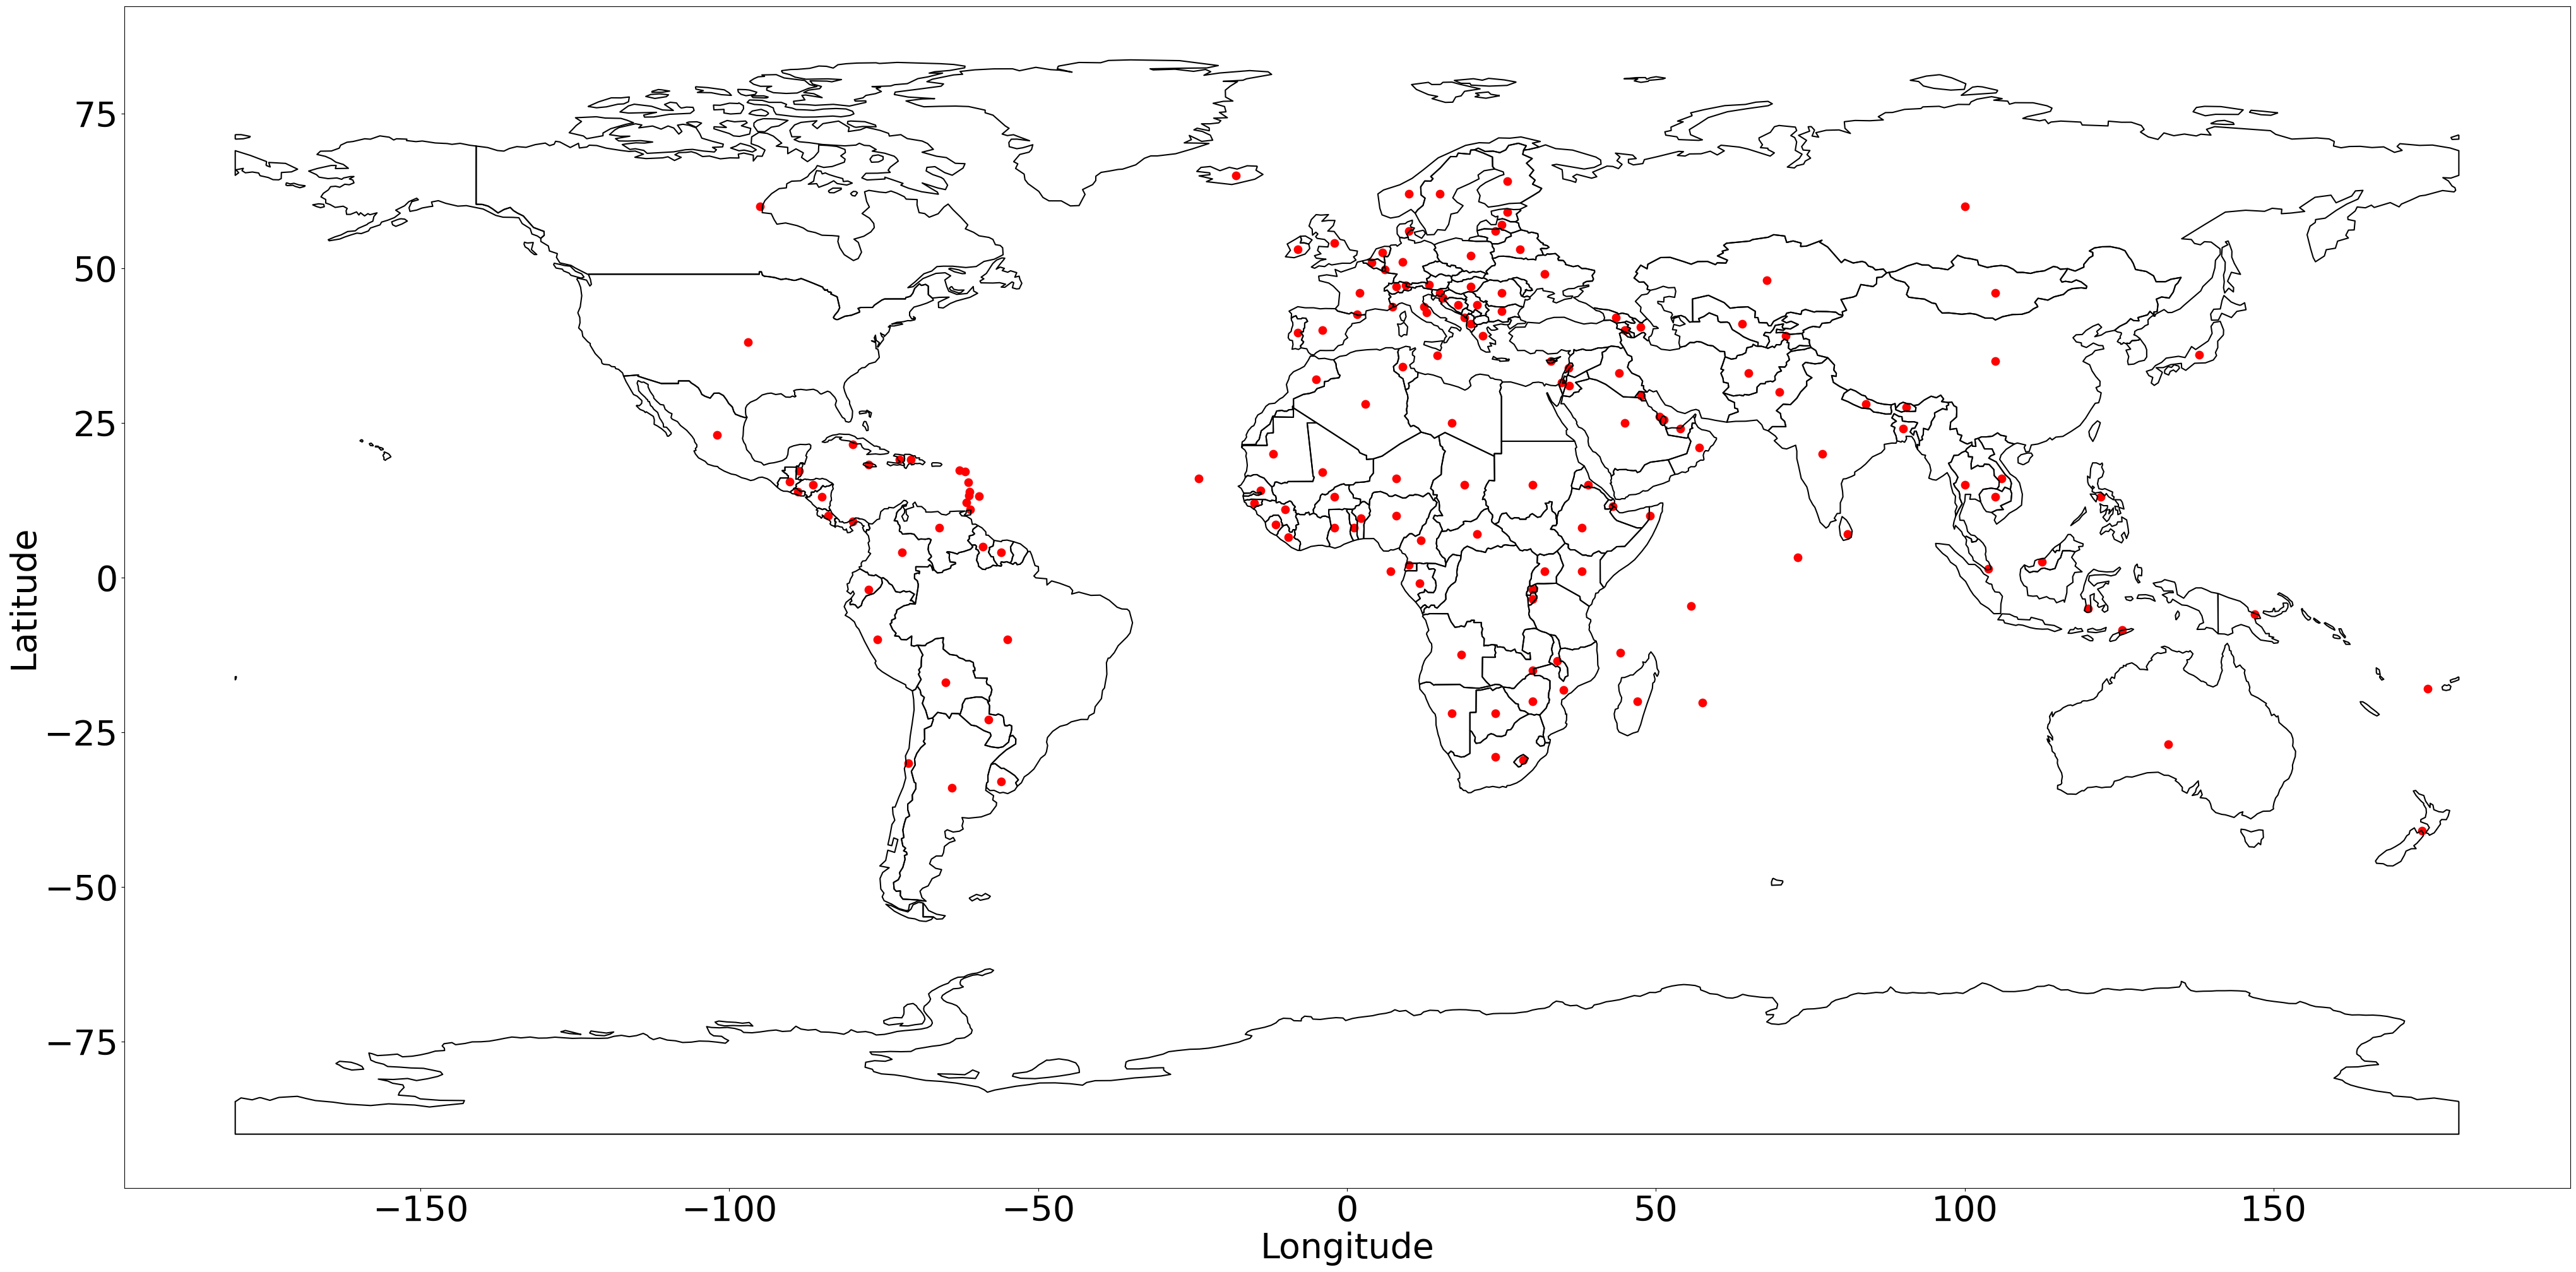
\includegraphics[width=\columnwidth]{img/loc_world.png}
    \caption{Position des pays sur la carte du monde}
    \label{fig:loc_world}
\end{figure}

Comme on le constate pour le Canada par exemple, le point qui le représente est situé
à une localisation étrange mais qui correspond bien à la latitude et la longitude moyenne
du pays. Plus le pays a une forme concave, plus le point risque d'être en dehors des
frontières du pays mais nous n'avons pas vraiment de méthode plus représentative à notre
disposition.
\\

\subsubsection{Population urbaine}\hfill\\

La part de population urbaine est calculée comme suit :
$$ R = \frac{U}{T} $$ où $U$ est la population urbaine et $T$ la population totale.

Voici la distribution de la part de population urbaine pour les pays étudiés. (fig. \ref{fig:urb_rate})

\begin{figure}[h]
    \centering
    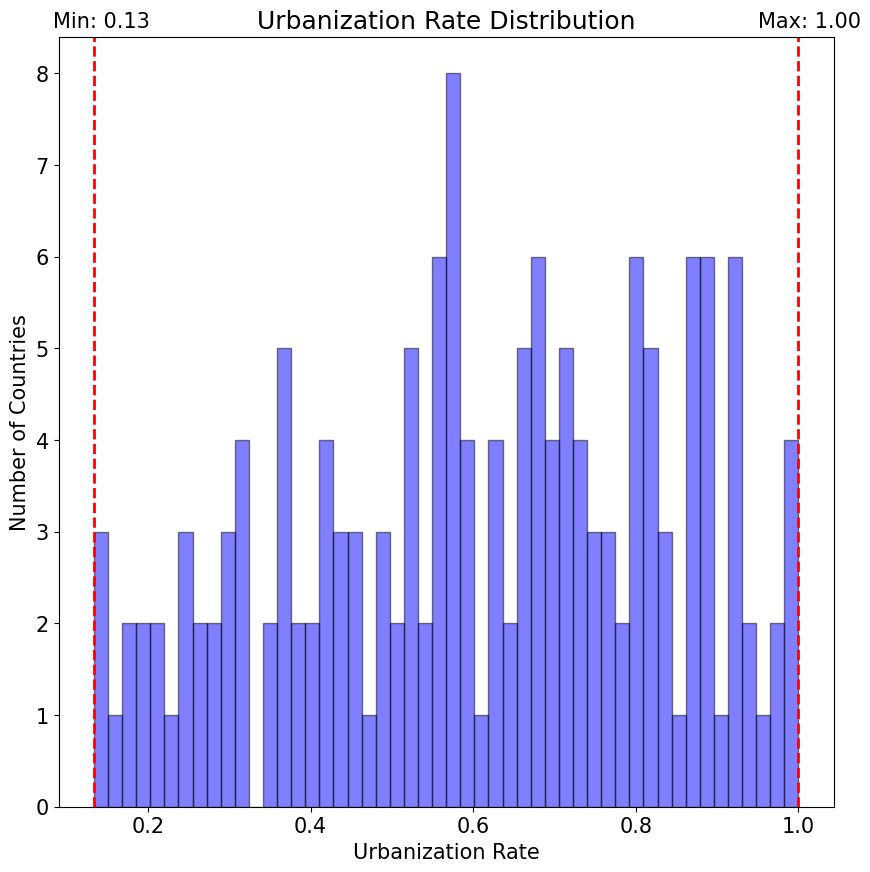
\includegraphics[width=6cm]{img/urb_rate.png}
    \caption{Distribution de la part de population urbaine}
    \label{fig:urb_rate}
\end{figure}

On constate que le taux de population urbaine est bien compris entre 0 et 1 pour tous les pays
et que la distribution est assez uniforme, avec légèrement plus de pays ayant une part de population
urbaine élevée.

On peut également visualiser le taux de population urbaine sur un planisphère. (fig. \ref{fig:urb_rate_world})

\begin{figure}[h]
    \centering
    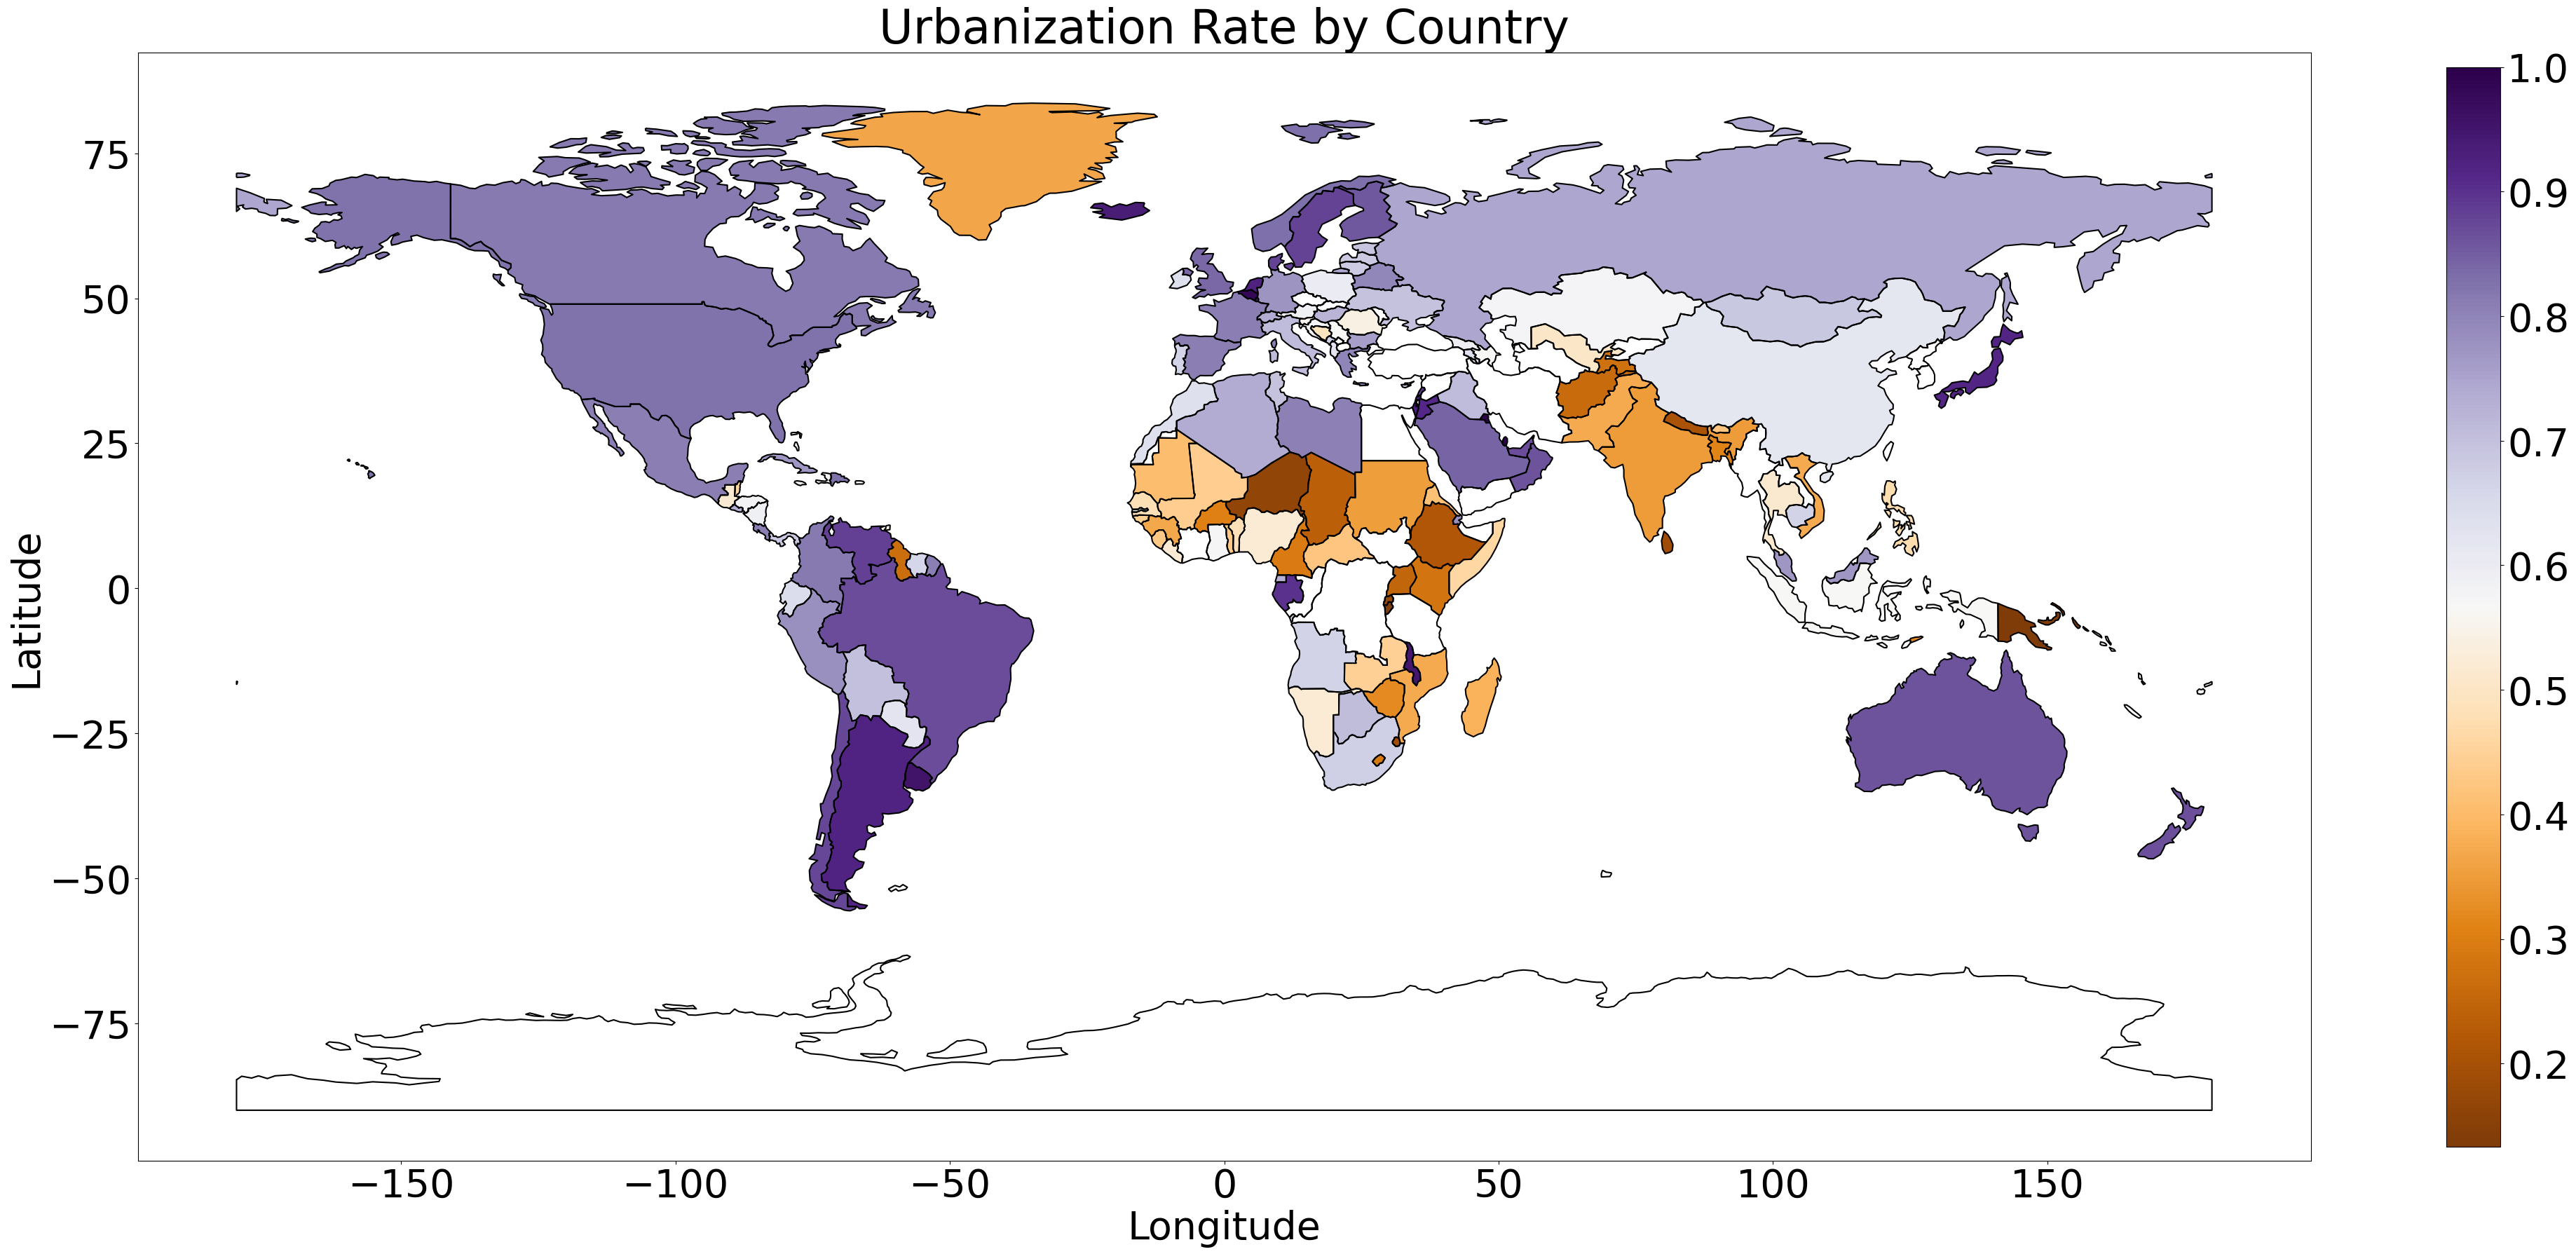
\includegraphics[width=\columnwidth]{img/urb_rate_world.png}
    \caption{Taux de population urbaine dans le monde}
    \label{fig:urb_rate_world}
\end{figure}

Comme on pouvait s'y attendre, les pays les plus urbanisés sont ceux qui sont
les plus développés. On constate ainsi que l'Afrique est le continent le moins
urbanisé et que l'Asie du Sud est également peu urbanisée.
\\

\subsubsection{Température moyenne}\hfill\\

La température moyenne dans le monde est de 18.2°C. Cependant la distribution des températures
moyennes est très large puisqu'elle va de -5.35°C à 28.29°C. Cette distribution semble
bimodale avec un pic autour de 10°C et un autre autour de 25°C. (fig. \ref{fig:temp})

\begin{figure}[h]
    \centering
    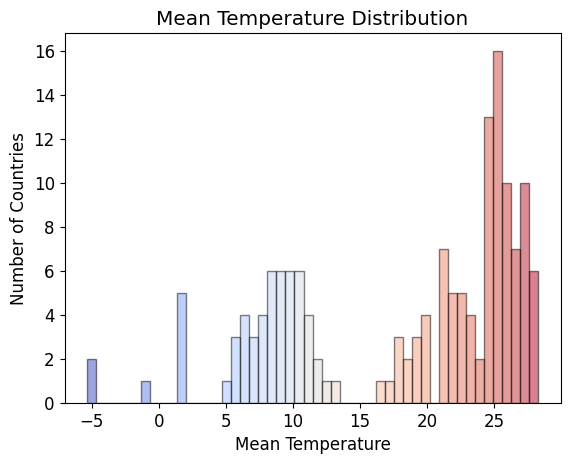
\includegraphics[width=6cm]{img/temp.png}
    \caption{Distribution de la température moyenne}
    \label{fig:temp}
\end{figure}

En visualisant la température moyenne sur un planisphère, on constate que les pays les plus
chauds sont situés autour de l'équateur et que les pays les plus froids sont situés près des
pôles. Également, les données semblent cohérentes puisque les pays proches les uns des autres
ont des températures similaires. (fig. \ref{fig:temp_world})

Les pays en blanc sont ceux pour lesquels nous n'avons pas de donnée.

\begin{figure}[h]
    \centering
    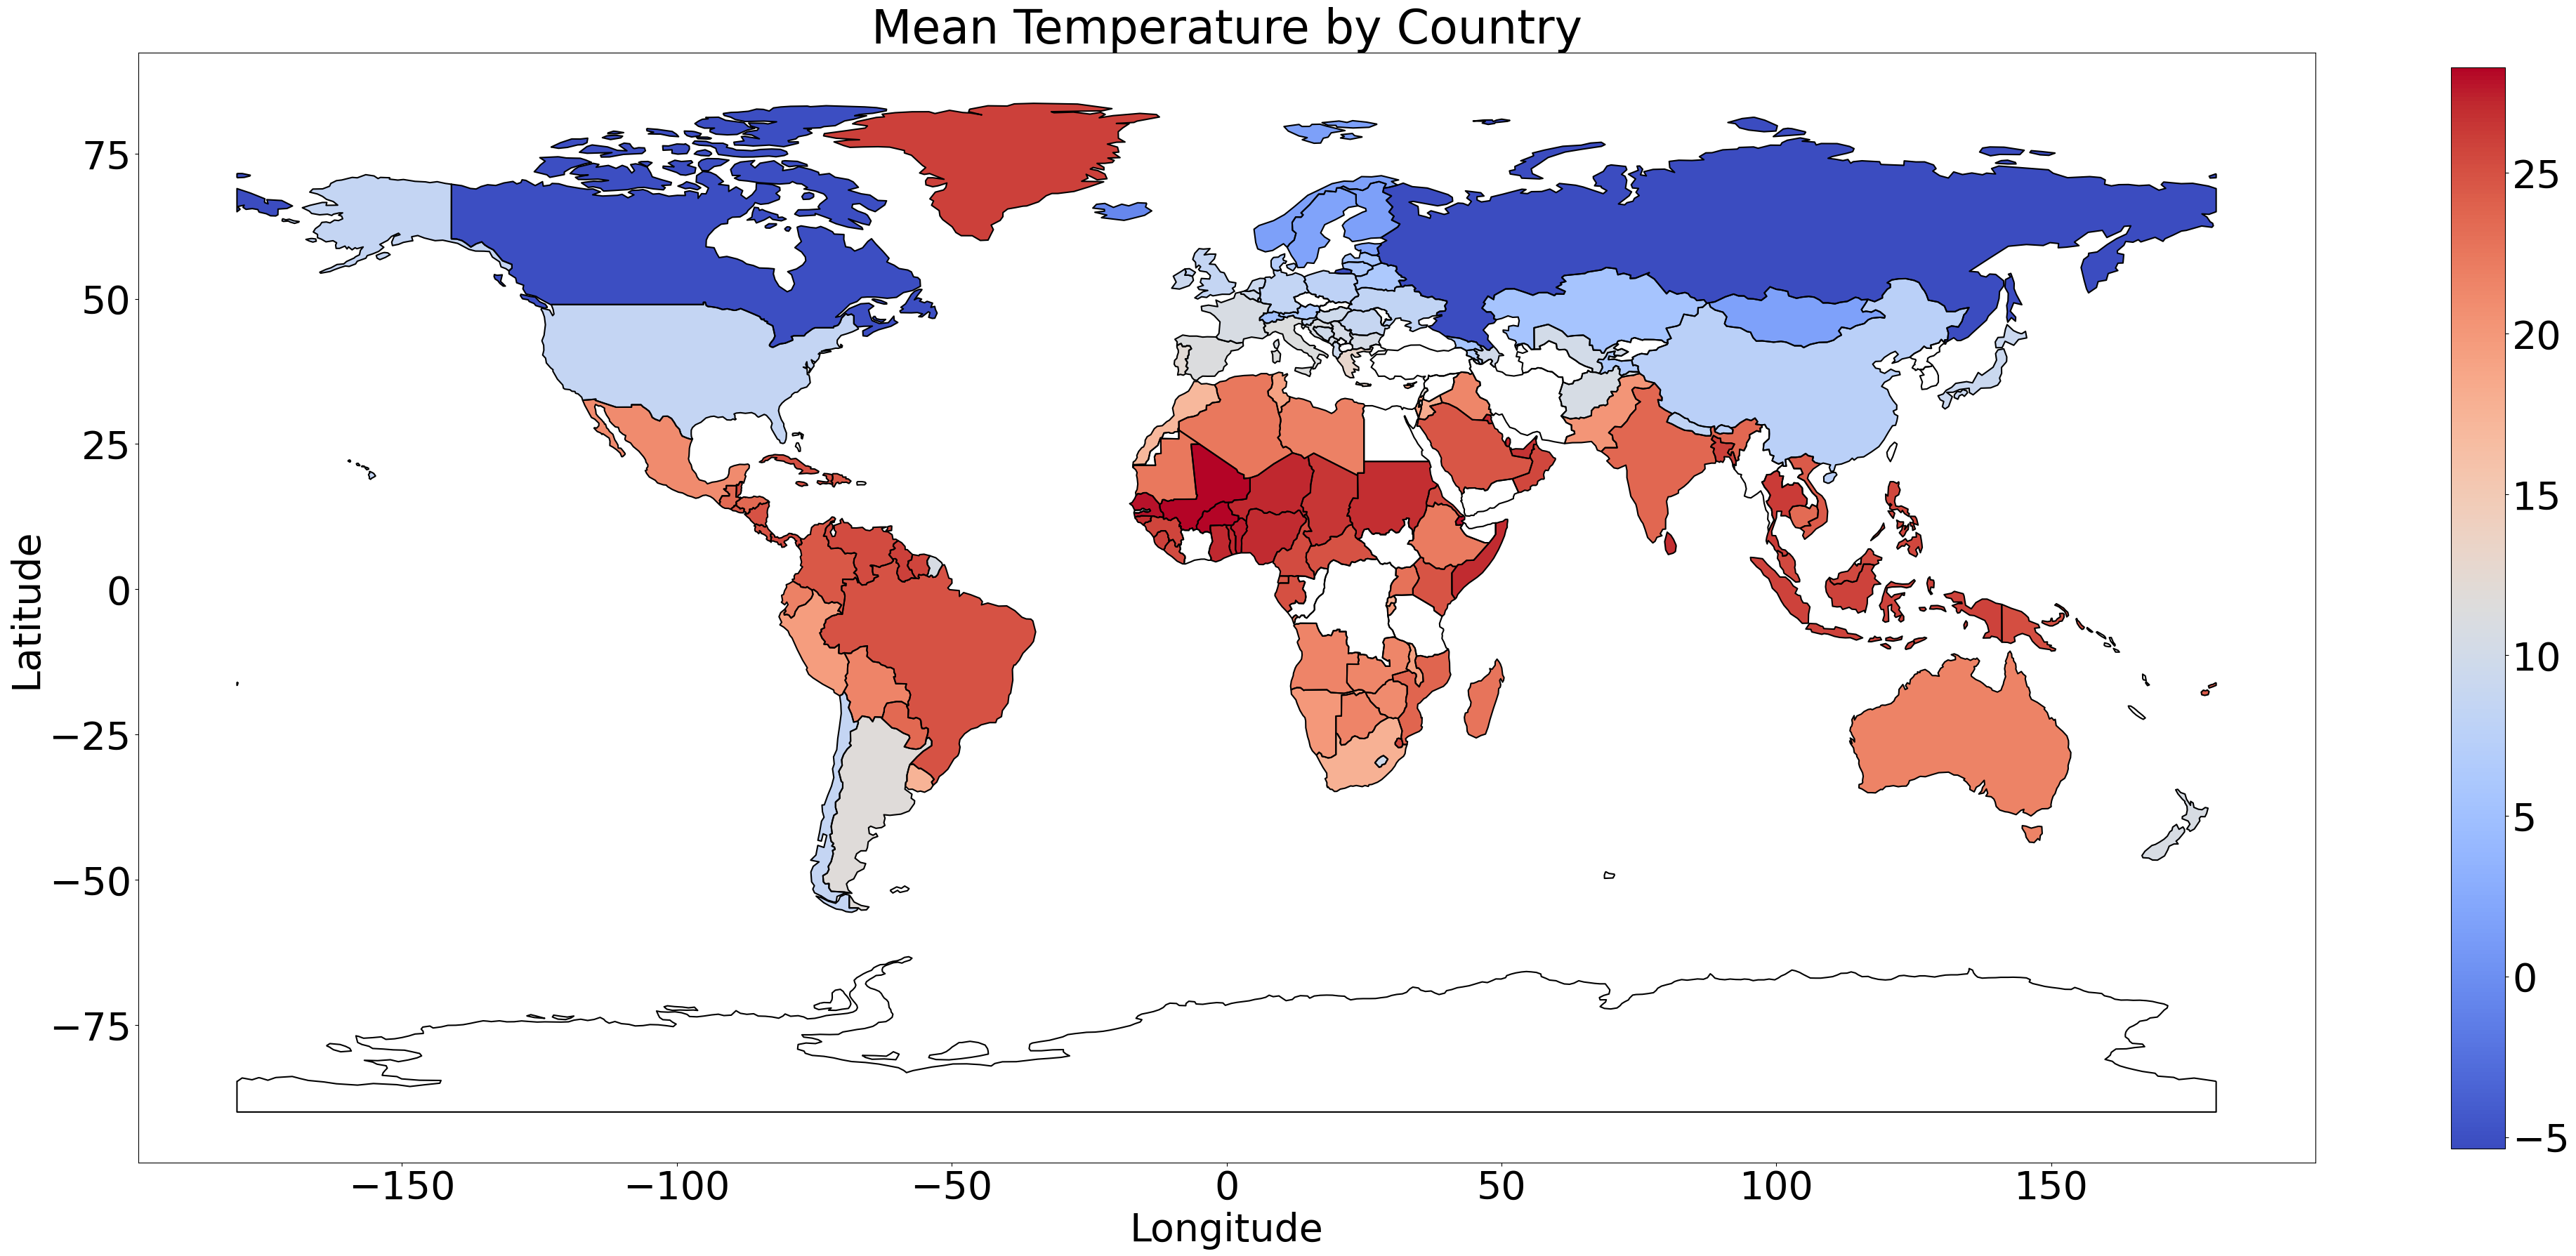
\includegraphics[width=\columnwidth]{img/temp_world.png}
    \caption{Température moyenne dans le monde}
    \label{fig:temp_world}
\end{figure}

\subsection{Problématique}
La propagation du COVID-19 est-elle vraiment liée à la position géographique des pays
et est-elle liée à d'autres facteurs comme la densité de population ou le climat ?

\subsection{Historique des travaux et développements}
Comme évoqué précédemment, une étude \cite{kaggle} a déjà été réalisée sur la relation entre
la propagation du virus et la latitude. Cette étude utilisait comme indicateur de la propagation
le taux de mortalité. Cependant, de nombreuses critiques ont mentionné que cette étude ne prenait
pas assez de facteurs en compte et donc que les résultats obtenus n'étaient pas suffisants pour
conclure que la position géographique était un facteur déterminant dans la propagation du virus.

\newpage
\section{Algorithmes}
\subsection{Calcul de la propagation du virus}

Nous avons à notre disposition des séries temporelles de cas confirmés de COVID-19 pour chaque
pays, il nous a fallu en extraire un indicateur de propagation du virus sous la forme d'un
unique nombre par pays.
\\

\subsubsection{Troncature des courbes}\hfill\\
En observant les séries temporelles et en les comparant aux manières dont a été gérée la pandémie
dans les différents pays, on constate que les mesures prises par les gouvernements (port du masque,
confinement, campagnes de vaccination, etc.) ont eu un impact sur la propagation du virus.

Afin d'extraire un indicateur de propagation comparable entre les pays, nous avons essayé de tronquer
les courbes de cas confirmés pour ne considérer que les périodes où le virus se propageait de manière
naturelle, c'est-à-dire avant que les mesures gouvernementales n'aient un impact significatif.

Pour ce faire nous avons d'abord lissé les courbes en utilisant une moyenne mobile car les données sont
très bruitées et que pour cette partie de l'analyse, nous ne cherchons pas à être précis mais plutôt à
capturer les grandes tendances. (fig. \ref{fig:moving_avg})

\begin{figure}[h]
    \centering
    \includegraphics[width=\columnwidth]{img/moving_avg.png}
    \caption{Cas confirmés et dérivée, sans et avec moyenne mobile}
    \label{fig:moving_avg}
\end{figure}

Nous avons ensuite essayé de tronquer les courbes avec la bibliothèque Python \texttt{ruptures} qui
permet de détecter des points singuliers d'une courbe mais nous ne sommes pas parvenus à trouver
des paramètres qui nous donnaient des résultats satisfaisants sur l'ensemble des pays.

Pour détecter les changements de tendance dans la propagation du virus, nous avons calculé la dérivée
des courbes de cas confirmés. La dérivée d'une série temporelle représente la variation entre chaque point
de données et le point précédent. Nous avons repéré le point où la dérivée était maximale, ce qui
correspond au pic de propagation du virus. Ensuite, en remontant dans le temps à partir de ce point,
nous avons tronqué la courbe aux endroits où la dérivée passait en dessous d'un premier seuil fixé à 5\%.
Nous avons procédé de la même manière en avançant dans le temps à partir du pic, en tronquant la courbe
lorsque la dérivée descendait sous un second seuil de 70\%. (fig. \ref{fig:clip})

Les seuils ont été choisis de manière empirique en observant les résultats produits sur un échantillon de pays
avec des courbes variées. (fig. \ref{fig:clip_full})

\begin{figure}[h]
    \centering
    \includegraphics[width=\columnwidth]{img/clip.png}
    \caption{Exemple de troncature, cas de la France}
    \label{fig:clip}
\end{figure}

\subsubsection{Calcul du facteur de propagation}\hfill\\
Il a ensuite fallu extraire des portions de courbes conservées un indicateur de propagation du virus
pour chaque pays. Nous avons testé quatre méthodes différentes :
\begin{itemize}
    \item Régression linéaire
    \item Régression exponentielle
    \item Temps nécessaire pour doubler le nombre de cas
    \item Ratio de reproduction quotidien
\end{itemize}

\vskip 0.3cm
\noindent\textbf{Régression linéaire} : 

Nous avons ajusté une droite de la forme $y = ax + b$ sur les données de cas confirmés en utilisant
la bibliothèque Python \texttt{scikit-learn} et avons pris le coefficient $a$ comme indicateur de
propagation.

\begin{figure}[h]
    \centering
    \includegraphics[width=\columnwidth]{img/lin_reg.png}
    \caption{Régression linéaire}

    \label{fig:lin_reg}
\end{figure}

Comme on peut le voir sur la figure \ref{fig:lin_reg}, la régression linéaire ne semble pas être un
bon modèle lorsqu'il s'agit de modéliser la propagation d'un virus. Dans le cas de certains pays, la
droite est proche de la courbe, mais pour la pluaprt ce n'est pas le cas et le coefficient directeur
est sensible à la population totale du pays ce qui n'est pas souhaitable.
\\

\noindent\textbf{Régression exponentielle} :

Nous avons ajusté une courbe de la forme $y = e^{ax+b}$ sur les données de cas confirmés en utilisant
la bibliothèque Python \texttt{scipy} et avons pris le coefficient $a$ comme indicateur de propagation.

Nous nous sommes assurés de translater les courbes tronquées pour que le premier point de la série
aient une ordonnée de 0 avant de faire la régression, et nous avons ensuite translaté la courbe
résultant de la régression pour qu'elle corresponde à la courbe originale.

\begin{figure}[h]
    \centering
    \includegraphics[width=\columnwidth]{img/exp_reg.png}
    \caption{Régression exponentielle}

    \label{fig:exp_reg}
\end{figure}

Comme on peut le voir sur la figure \ref{fig:exp_reg}, la régression exponentielle semble donner
des résultats satisfaisants sur différents types de courbes.

Nous avons appliqué un min-max scaling sur les coefficients obtenus pour chaque pays afin de les
ramener entre 0 et 1 et de pouvoir les comparer.
\\

\noindent\textbf{Nombre moyen de jours requis pour doubler le nombre de cas} :

Une autre manière de calculer le taux de propagation est de calculer le temps qu'il faut pour que le nombre
de cas confirmés double. Cette méthode est robuste à la forme de la courbe et facile à calculer mais puisque
nous avons tronqué les séries temporelles à un certain point, l'initialisation ne sera pas la même pour chaque
pays même après translation. Certains pays pourraient déjà avoir gagné un certain élan au début de la série
temporelle tronquée et cela ferait que le temps pour doubler les cas serait plus petit qu'il ne devrait l'être.

Pour éviter cela, nous avons décidé de ne prendre en compte le temps pour doubler les cas qu'à partir
d'une certaine portion de la série temporelle en espérant que le taux de propagation se soit stabilisé.

Ainsi, nous avons choisi de ne considérer que les derniers 75\% de la série temporelle tronquée.

\begin{figure}[h]
    \centering
    \includegraphics[width=\columnwidth]{img/time_double.png}
    \caption{Temps pour doubler les cas}

    \label{fig:time_double}
\end{figure}

Comme on peut le voir sur la figure \ref{fig:time_double}, notre manipulation a permis de stabiliser
le temps pour doubler les cas pour chaque pays et de minimiser l'impact de l'initialisation.

Pour ramener cet indicateur entre 0 et 1, nous avons utilisé la formule suivante :
$$v' = \frac{v_{max}-v}{v_{max}}$$ où $v_{max}$ est le temps pour doubler les cas le plus grand parmi
tous les pays.
\\

\noindent\textbf{Ratio de reproduction quotidien} :

Cette méthode consiste à calculer l'augmentation relative moyenne du nombre de cas confirmés par jour
sur la période considérée. C'est une méthode simple et intuitive qui semble fonctionner correctement.
Nous avons, comme pour l'indicateur précédent, décidé de ne considérer que les derniers 75\% de la série
temporelle tronquée.

La formule utilisée est la suivante :
$$v = \frac{1}{n-1} \sum_{i=1}^{n-1} \frac{c_{i+1} - c_i}{c_i}$$ où $c_i$ est le nombre de cas confirmés
au jour $i$ et $n$ est le nombre de jours considérés.

À nouveau, un min-max scaling a été appliqué pour ramener les valeurs entre 0 et 1.

Voici les valeurs que l'on obtient pour quelques pays :
\begin{table}[h]
    \centering
    \begin{tabular}{|c|c|}
        \hline
        Pays & Ratio de reproduction quotidien \\
        \hline
        France & 0.052 \\
        United Kingdom & 0.042 \\
        United States & 0.015 \\
        China & 0.098 \\
        Russia & 0.031 \\
        Ethiopia & 0.035 \\
        Afghanistan & 0.052 \\
        \hline
    \end{tabular}
\end{table}

\newpage

\noindent\textbf{Comparaison des méthodes} :

Afin de comparer les différentes méthodes, nous avons affiché les positions de quelques
pays pour chacune d'entre elles. (fig. \ref{fig:spread_comp})

\begin{figure}[h]
    \centering
    \includegraphics[width=\columnwidth]{img/spread_comp.png}
    \caption{Comparaison des méthodes de calcul de la propagation}

    \label{fig:spread_comp}
\end{figure}

On constate notamment que le temps moyen pour doubler les cas présente un classement assez
différent des deux autres méthodes.

En calculant les corrélations deux à deux entre les différents indicateurs (Régression exponentielle (exp),
Temps pour doubler les cas (T2C) et Ratio de reproduction quotidien (repr)), on obtient les
valeurs suivantes qui corroborent les observations faites sur les graphiques :

\begin{table}[h]
    \centering
    \begin{tabular}{|c|c|c|c|}
        \hline
        corr & exp & T2D & repr \\
        \hline
        exp & 1.0 & 0.43 & 0.78 \\
        T2C & 0.43 & 1.0 & 0.61 \\
        repr & 0.78 & 0.61 & 1.0 \\
        \hline
    \end{tabular}
\end{table}

Après avoir comparé les résultats de la régression exponentielle et du ratio de reproduction
quotidien entre eux et avec les courbes, nous avons décidé de poursuivre notre étude en
utilisant le coefficient de le ratio de reproduction quotidien comme indicateur de propagation
car il semble être moins sensible à la forme des courbes et donne des résultats plus cohérents
dans l'ensemble.

\newpage
\subsection{Résultats et interprétation}

\subsubsection{Comparaison entre le taux de mortalité et le taux de propagation}\hfill\\

Pour commencer, nous pouvons comparer notre taux de propagation avec le taux de mortalité
utilisé dans l'étude précédente \cite{kaggle}.

\begin{figure}[h]
    \centering
    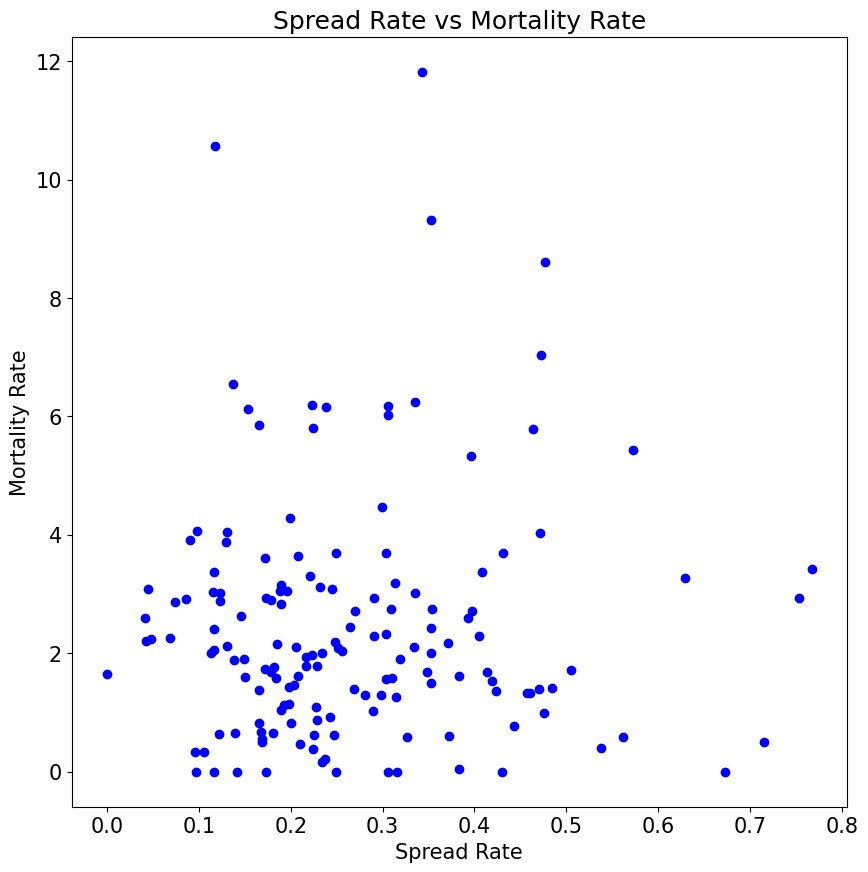
\includegraphics[width=6cm]{img/spread_mort_corr.png}
    \caption{Comparaison du taux de mortalité et du taux de propagation}

    \label{fig:spread_mort_corr}
\end{figure}

On constate (fig. \ref{fig:spread_mort_corr}) que le taux de mortalité et le taux de propagation
ont des distributions assez différentes.

La corrélation entre les deux indicateurs est de 0.04, ce qui confirme que le taux de mortalité
n'est pas un bon indicateur de la propagation du virus.
\\
\\

\subsubsection{Corrélation entre la position et la propagation}\hfill\\

Nous avons essayé de reproduire les résultats de l'étude précédente \cite{kaggle} en comparant
la valeur absolue de la latitude des pays avec leur taux de mortalité d'abord puis avec notre taux de propagation.

\begin{figure}[h]
    \centering
    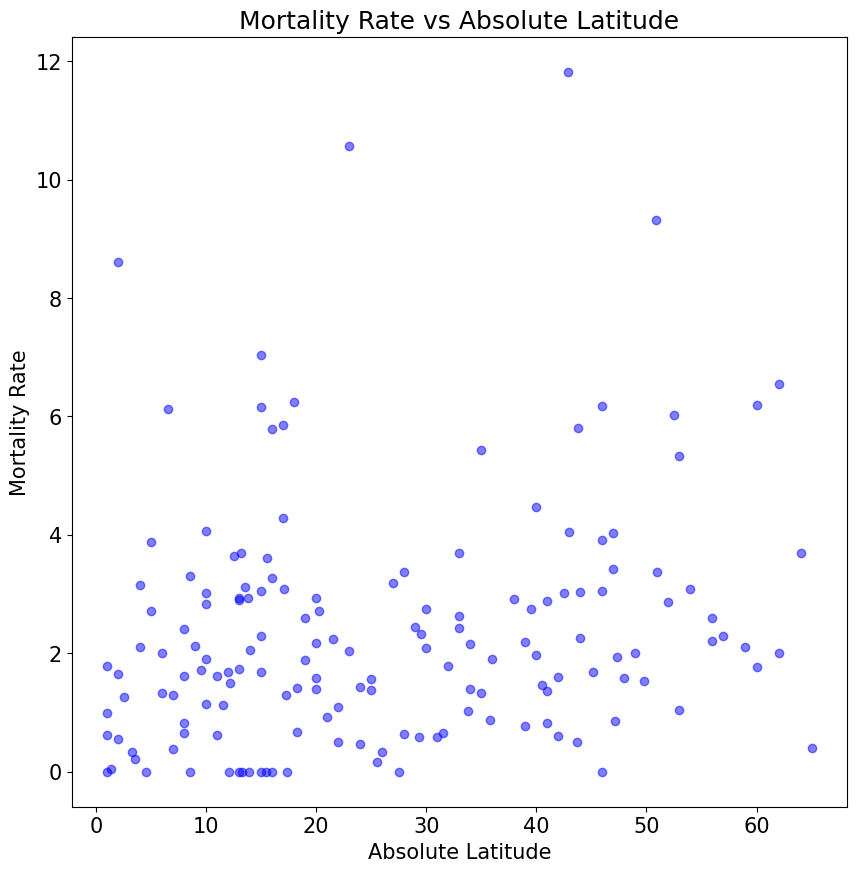
\includegraphics[width=6cm]{img/mort_lat.png}
    \caption{Latitude absolue vs. taux de mortalité}
    \label{fig:mort_lat}
\end{figure}

On obtient une corrélation assez faible de 0.20 et un graphe (fig. \ref{fig:mort_lat})
qui est bien identique à celui présenté dans notre étude de référence.

Dans cette étude, l'auteur utilise également l'argument d'une corrélation plus élevée
au sein des États-Unis pour affirmer que la latitude est un facteur important dans la
propagation du virus. Comme nous le voyons à l'échelle du monde, cette corrélation
est faible et il nous semble plus probable que d'autres facteurs entrent en jeu.

Dans
cette étude, les données de cas confirmés ne sont pas tronquées et il est donc possible
que les mesures gouvernementales aient un impact sur les résultats, surtout dans un pays
comme les États-Unis qui est connu pour avoir une politique très hétérogène entre les 
états du Nord et du Sud.

En utilisant notre indicateur de propagation, nous obtenons une corrélation encore
plus faible de 0.04 et la distribution est encore plus uniforme. (fig. \ref{fig:spread_lat})

\begin{figure}[h]
    \centering
    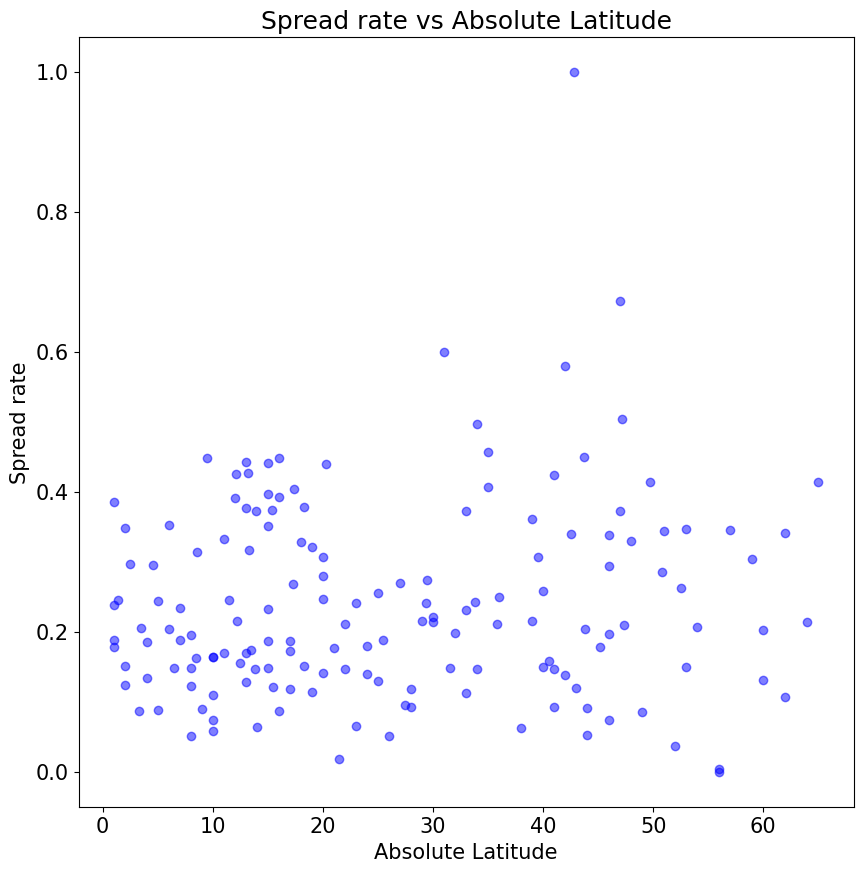
\includegraphics[width=6cm]{img/spread_lat.png}
    \caption{Latitude absolue vs. taux de propagation}
    \label{fig:spread_lat}
\end{figure}

La corrélation avec la longitude valant 0.006 (fig. \ref{fig:spread_lon}), nous pouvons conclure que la position
géographique n'est pas un facteur déterminant dans la propagation du virus.

\newpage

\subsubsection{Corrélation entre la part de population urbaine et la propagation}\hfill\\

Nous avons ensuite comparé la part de population urbaine des pays avec notre taux de propagation. (fig. \ref{fig:spread_urb_rate})

\begin{figure}[h]
    \centering
    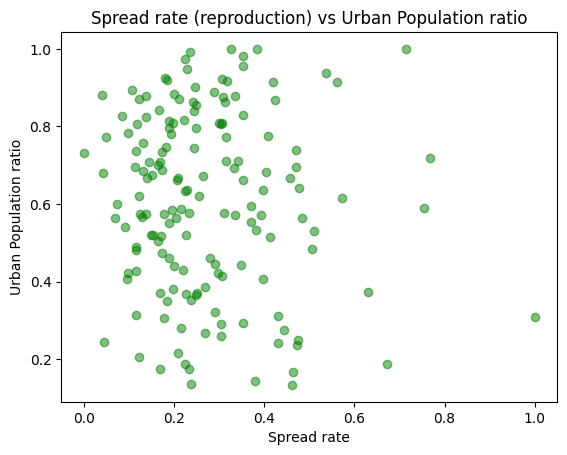
\includegraphics[width=6cm]{img/spread_urb_rate.png}
    \caption{Taux de propagation vs. part de population urbaine}
    \label{fig:spread_urb_rate}
\end{figure}

La corrélation correspondante est de -0.08, ce qui est faible et semble indiquer que la part de population
urbaine n'est pas un facteur déterminant dans la propagation du virus bien que nous nous serions
plutôt attendus à une corrélation positive et assez importante.

Pour illustrer cette non-corrélation, nous avons calculé le nombre de pays se situant dans les
différents quartiles de part de population urbaine et de taux de propagation.

Voici les résultats obtenus :

\begin{table}[h]
    \centering
    \begin{tabular}{|c|c|c|}
        \hline
        & Q1 urb. & Q4 urb. \\
        \hline
        Q1 prop. & 8 & 8 \\
        \hline
        Q4 prop. & 13 & 8 \\
        \hline
    \end{tabular}
\end{table}

On compte ainsi un total de 16 pays supportant la thèse d'une corrélation positive 
(la somme de la diagonale principale) et 21 pays supportant la thèse d'une corrélation négative
(la somme de l'anti-diagonale). Cela semble confirmer que ni l'une ni l'autre
de ces hypothèses n'est correcte, d'autant plus que seuls 37 pays sur 159 apparraissent dans
ces résultats et que donc la majorité des pays ne se retrouvent dans aucune de ces hypothèses.
\\

\subsubsection{Corrélation entre le climat et la propagation}\hfill\\

Enfin, nous avons comparé la classification climatique de Köppen-Geiger et la température moyenne
des pays avec notre taux de propagation.

Nous avons commencé par utiliser la classification brute que nous avons calculé pour chaque pays. (fig. \ref{fig:spread_clim})

\begin{figure}[h]
    \centering
    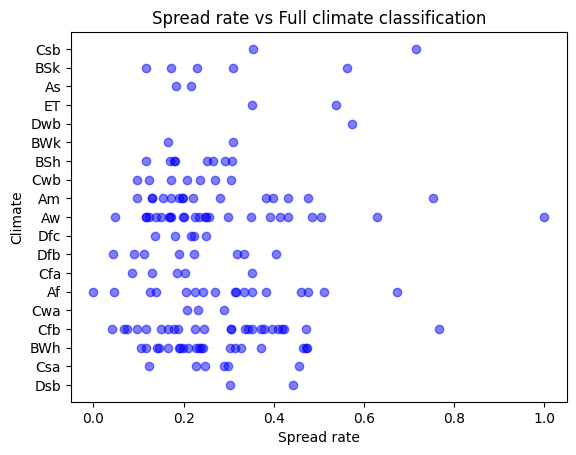
\includegraphics[width=6cm]{img/spread_clim.png}
    \caption{Taux de propagation vs. classification climatique}
    \label{fig:spread_clim}
\end{figure}

La corrélation correspondante étant très basse (-0.02), nous avons décidé d'isoler les
différentes caractéristiques qui composent cette classification pour voir si l'une d'entre
elles était plus corrélée à la propagation du virus.

La première lettre de la classification de Köppen-Geiger correspond au climat principal
du pays. Nous avons donc comparé cette lettre avec notre taux de propagation. (fig. \ref{fig:spread_main_clim})

\begin{figure}[h]
    \centering
    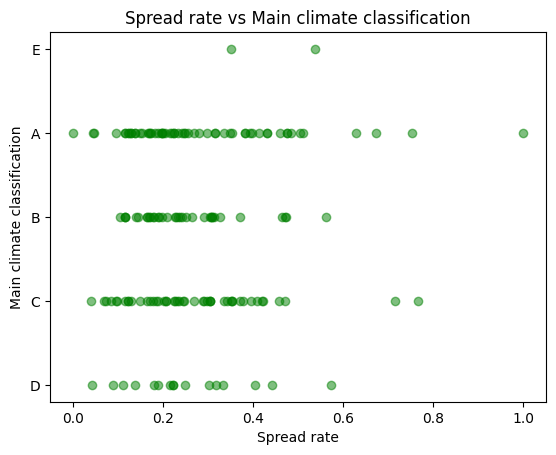
\includegraphics[width=6cm]{img/spread_main_clim.png}
    \caption{Taux de propagation vs. climat principal}
    \label{fig:spread_main_clim}
\end{figure}

La corrélation correspondante est de -0.03, ce qui est très faible et semble indiquer que le climat
principal n'est pas un facteur déterminant dans la propagation du virus.

Nous avons ensuite comparé le type de précipitations avec notre taux de propagation. (fig. \ref{fig:spread_prec})

\begin{figure}[h]
    \centering
    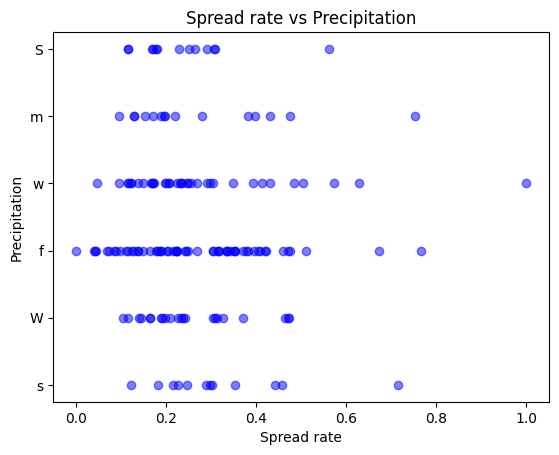
\includegraphics[width=6cm]{img/spread_prec.png}
    \caption{Taux de propagation vs. type de précipitations}
    \label{fig:spread_prec}
\end{figure}

La corrélation correspondante est un peu plus élevée (0.09) mais toujours insuffisante pour conclure
que le type de précipitations serait un bon prédictif de la propagation du virus.

Enfin, nous avons comparé la composante de température de la classification avec notre taux de propagation.
(fig. \ref{fig:spread_temp})

\begin{figure}[h]
    \centering
    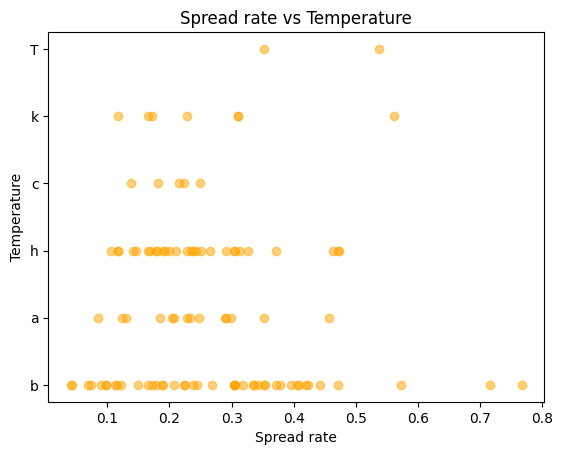
\includegraphics[width=6cm]{img/spread_temp.png}
    \caption{Taux de propagation vs. type de température}
    \label{fig:spread_temp}
\end{figure}

Là encore, une corrélation de -0.09 semble montrer que le type de température n'est pas un bon indicateur
de la propagation du virus.

Nous avons également comparé la température moyenne des pays avec notre taux de propagation. (fig. \ref{fig:spread_mean_temp})

\begin{figure}[h]
    \centering
    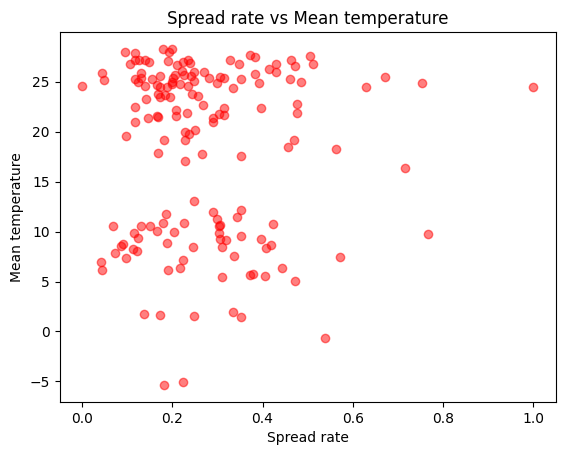
\includegraphics[width=6cm]{img/spread_mean_temp.png}
    \caption{Taux de propagation vs. température moyenne}
    \label{fig:spread_mean_temp}
\end{figure}

La corrélation correspondante étant nulle, on peut sans trop de risque conclure que la température
n'est pas liée à notre taux de propagation.

\subsection{Applications concrètes}
Malgré l'absence de bon prédictif de la propagation du virus parmi les variables que nous avons
étudiées, notre étude à permis de réfuter l'hypothèse que la position géographique serait un facteur
déterminant dans la propagation du virus.

Cela participe à améliorer notre compréhension de la propagation des virus et permet de mettre
en lumière l'importance de prendre en compte plusieurs facteurs pour pouvoir prédire la propagation
d'une maladie infectieuse.

On se rend également compte que même si l'étude précédente annonçait une corrélation entre la latitude
et la propagation du virus et que celle-ci n'était déjà pas très élevée aux États-Unis, une étude
plus appronfondie à l'échelle mondiale aurait pu mettre l'auteur sur la piste que d'autres facteurs
pourraient être en jeu, soulignant l'importance de garder un esprit critique et de ne pas se reposer
sur des résultats sans les remettre en question.

\subsection{Limites}
Nous avons été limités par la qualité des données disponibles. En effet, certaines données
ne sont disponibles que par pays et d'autres pour des points du globe. Nous avons donc dû
faire des approximations pour pouvoir les utiliser. Ce point pose notamment problème pour
la classification climatique de Köppen-Geiger qui est disponible pour des points du globe et
peut différer d'une région à l'autre d'un même pays. Également, les données de COVID-19
ne sont disponibles qu'à l'échelle des pays ou de grandes régions, ce qui ne nous permet
pas de faire des analyses plus fines quant aux différences d'urbanisation ou de climat
à l'intérieur d'un même pays.

Les information lacunaires sur les cas confirmés de COVID-19 ont également rendu difficile
la détermination d'un bon indicateur de propagation du virus. Ce genre d'étude est normalement
réalisé à l'échelle nationale et non mondiale, en fonction de toutes les politiques
mises en place par le pays et en prédisant précisément l'impact qu'elles auront
afin de garder une continuité dans les calculs qui sont fait tout au long de l'épidémie.
Dans nos cas, nous avons dû tronquer les courbes de cas confirmés avec une méthode 
systématique car nous ne pouvions pas prendre en compte les politiques des 159 pays
un par un.

Dans le cas du calcul du R0 par exemple, il
est nécessaire de prendre en compte des dizaines de paramètres inaccessibles en ligne
pour obtenir un résultat fiable et même dans ce cas,
le R0 évolue rapidement au cours d'une épidémie. 

En résumé, la précision insuffisante des données et la complexité du problème nous pousse
à faire des approximations qui ont probablement complétement obscurci les
conclusions que nous aurions pu tirer de cette étude.

\subsection{Conclusion}

Nous sommes parvenus à réfuter l'hypothèse que la position géographique était un facteur
déterminant dans la propagation du virus ce qui était la motivation première de notre étude.

Les résultats plus généraux à l'échelle mondiale que nous aurions souhaité obtenir n'ont
pas pu être démontrés, probablement à cause de la qualité des données en libre accès
et de la complexité du problème. 

Pour aller plus loin, il serait peut-être intéressant de se pencher sur des études
plus locales, à l'échelle nationale par exemple, pour voir si des facteurs plus fins
comme la densité de population ou le climat local pourraient être des facteurs déterminants
dans la propagation du virus. Même dans ce cas cependant, il est probable que les données
disponibles en ligne ne soient pas suffisantes pour obtenir des résultats fiables.

\newpage
\bibliographystyle{plain}
\bibliography{bibliography}

\newpage

\section*{Annexes}
\renewcommand{\thefigure}{A\arabic{figure}}
\setcounter{figure}{0}

\begin{figure}[h]
    \centering
    \includegraphics[width=8cm]{img/clip_full.png}
    \caption{Troncature des courbes de cas confirmés}
    \label{fig:clip_full}
\end{figure}

\begin{figure}[h]
    \centering
    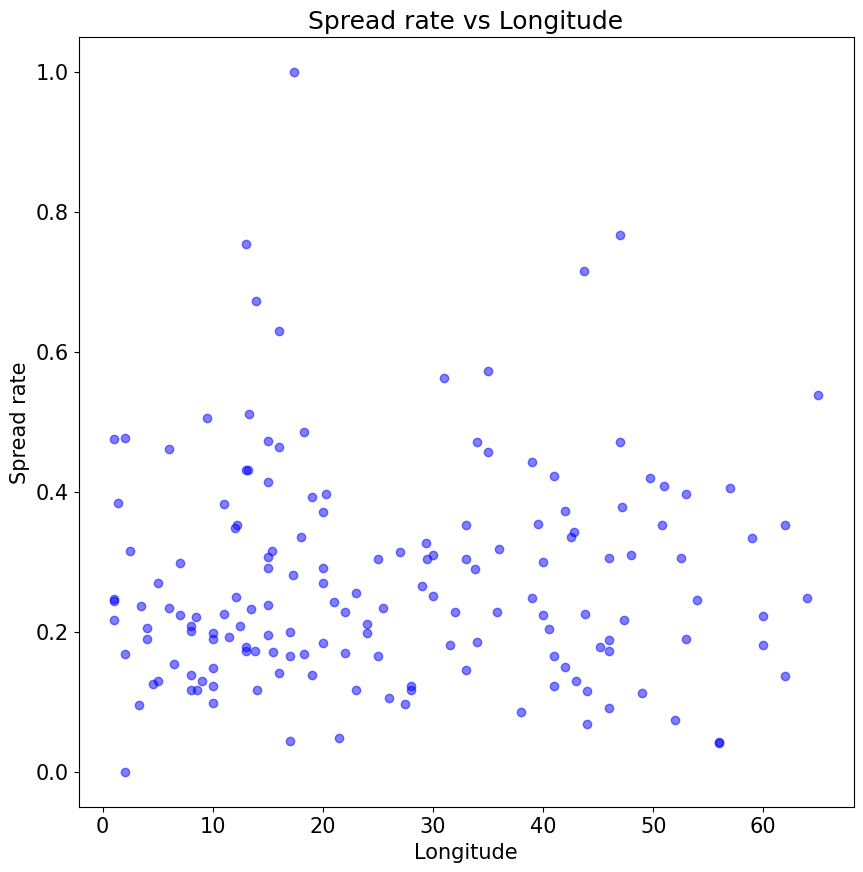
\includegraphics[width=8cm]{img/spread_lon.png}
    \caption{Longitude vs. taux de propagation}
    \label{fig:spread_lon}
\end{figure}

\end{document}